\section{Soll-Zustand}
Der Ist-Zustand im vorigen Kapitel hat gezeigt, dass viele manuelle Tätigkeiten für die Beladung und Abfertigung sowie die Rangiervorgänge von Güterwagen im Einzelwagenverkehr notwendig sind.\par
Dies verursacht hohe (Personal-)Kosten durch die benötigte Zeit und das benötigte Personal, sowie auch Kosten an der Verladestelle, wenn diese aufgrund von Kupplungs- und Rangiervorgängen still steht.\par
Bei einem Umbau für die Demonstratoren muss darauf geachtet werden, dass ein vollständiger Rückbau der neuen einrichtungen möglich ist, aber alls so bahntauglich ist, dass die Demonstratoren für ein Folgeprojekt oder Feldversuche genutzt werden können. Diese Projekt muss nicht sofort zulassungsfähig sein, sollte aber eine Basis dazu bilden. \par
An der Bewegung der Wagen im Wagenverband an sich mit Hilfe einer Lok oder eines anderen Rangierhilfsmittel kann nichts groß automatisiert werden. Siehe dazu auch Kapitel \ref{sec:Zustellfahrt}, \ref{sec:Zugfahrt} und \ref{sec:Rangierfahrt}. Automatisierungen können aber selbst verständlich im Bereich der Kupplung, Bremse oder auch der informationstechnischen Prozesse stattfinden.\par
Zur besseren Einordnung sollen nun einige Komponenten definiert und erläutert werden aus denen sich verschiedene Stufen ergeben und aus denen sich wiederum später verschiedene Anforderungen ergeben.

\subsection{Bremse}
\subsubsection{Parkbremse}
mit Lust = ungebremst, ohne Luft = gebremst
\subsubsection{Bremshundertstel/Bremsberechnung}
Die Bremshundertstel werden bisher, genau wie das Bremsgewicht, händisch mittels Bremszettel berechnet. \textbf{BILD}. Auf diesem Vordruck trägt der Triebfahrzeugführer Achszahl, Zugmasse und Bremsgewichte des Zuges ein. Daraus berechnen sich die Bremshundertstel. Nach Vergleich dieser mit den Mindest-Bremshundertstel der Strecke, ergibt sich Höchstgeschwindigkeit und Bremsstellung. die Bremsstellung wird nach jeder neuen Zusammenstellung und vor Fahrtantritt, siehe Kapitel \ref{sec:UEdWagen}, neu berechnet.\par
Diese manuelle Berechnung ist für Triebfahrzeugführer tägliche Arbeit, dennnoch ist sie Fehleranfällig und kann durch Rechnereinsatz einfach automatisiert werden.

\subsection{Kupplung}
Wie in Kapitel \ref{sec:Personal} angedeutet und in Kapitel \ref{sec:LuftumechKup} beschrieben, ist das mechanische Kuppeln und das Kuppeln von Luft aufwändig, körperlich anstrengend und fehlerbehaftet. \par
Zur Automatisierung von mechanischen Kupplungen gibt es Kupplungsrobotoren\footnote{Zum Beispiel die Bahn-Kupplungs-Robotoren BaKuRo und EntKuRo}, dort muss aber weiter händisch Luft gekuppelt werden \textbf{Ist das so?}. Alternativ ist die Automatische Kupplung eine Lösung, aber auch nach deren Einführung im vorigen Jahrhundert ist eine flächendeckende Nutzung im Güterverkehr noch nicht realisiert.\par
\textbf{Irgendwas zu Luft und elektrischen Ventilen.}\\
\textit{siehe auch \ref{sec:Vorpruefung} und \ref{sec:Zugvorbereitung}}
\par
Aufgrund dieser Punkte ist es erst einmal sinnvoll mich der mechanischen Kupplung weiter zu machen und Lösungen für die Automatische Kupplung kompatibel zu halten. Vor allem muss aber die Luftkupplung vereinfacht wreden wo es geht \textbf{ SIEHE AUCH: Luftventile.}

\subsection{Bewegung des Wagens}
In Kapitel \ref{sec:BewdWagen} werden die verschiedenen Möglichkeiten der Wagenbewegung betrachtet. Im Allgemeinen werden dafür zusätzliche Fahrzeuge, Personal und eine Gleisanlage benötigt. Je nach Beschaffung der Gleisanlage und die in Kapitel \ref{sec:Fahrweg} angesprochene Einschränkung, werden zusätzliche Sägefahrten zur korrekten Einsortierung der Wagen auf verschiedene Gleise benötigt. \par
Ein eigener Antrieb auf jedem Wagen, der eine selbstständige Bewegung in geringer Geschwindigkeit zulässt wäre hier eine Lösung.\par
\textit{\textbf{Probleme:} Stromversorgung, Akkuaufladung, Antrieb, Sicherheit}
\subsubsection{Adrücken}
DAs Abdrücken am Ablaufberg, siehe Kapitel \ref{sec:Abdruecken} ist bereits auf großen Rangierbahnhöfen automatisiert, siehe Kapitel \ref{sec:automAbdruecken}, dennoch ist auch dies Handarbeit zur Vorbereitung. Die Wagen müssen vorentkuppelt werden, sowohl mit der Luftkupplung, als auch mechanisch, dann aber wieder, mit einem Hemmschuh, festgelegt werden und kurz vorm Ablaufberg vollständig entkuppelt. 
Hemmschuh, vereinzeln, vorentkuppelt, Geschwindigkeit
\subsection{Sicherheit/Zugintegrität}
\subsubsection{Personalschulung}
Neue Systeme benötigen immer Zeit zur Einführung und Schulung des Personlas. Das gilt auch für dieses Projekt, aber auch jetzt schon sind die Handgriffe, wie in Kapitel \ref{sec:Personal} angesprochen, kompliziert und fehleranfällig. Durch informationstechnische Prozesse \textbf{MEHR DAZU UNTER}, die zusätzlich im Hintergrund laufen und durch weniger Handgriffe im üblichen Betrieb, sollen diese Prozesse einfacher und sicherer werden. Zusätzlich sollen die neu benötigten Handgriffe intuitiv zu den alten Handgriffen passen oder leicht erlenrnbar sein. Zusätzliches Schulungsmaterial soll leicht verständlich und intuitiv gestaltet werden.\par
\textit{\textbf{Probleme:} Annahme der Systeme, Kosten für die Schulung}

\subsection{Informationstechnische Prozesse}
\subsubsection{Bremsprobe}
\textbf{SIL-Bewertung - liegt nicht an, liegt an, sicheres lösen, sicheres stellen}.\par
Die \gls{Bremsprobe} findet zur Vorbereitung einer Sperr-, Rangier- oder Zugfahrt statt und überprüft die Funktionsfähigkeit des Bremssystems im Zug- oder Wagenverbund.\par
\begin{figure}[htbp] 
    \begin{center}
            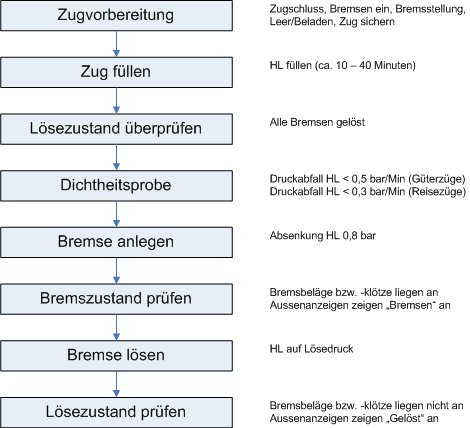
\includegraphics[width=9cm]{Bilder/bremsprobe.png}
            \caption{Schematische Übersicht der Bremsprobe}
            \label{fig:Bremsprobe}
    \end{center}
\end{figure} 
Sie wird von Bremsprobeberechtigten nach genau vorgeschriebenem Ablauf durchgeführt. Ja nach Zustand des Zuges und Fälligkeit der \gls{Bremsprobe} wird eine volle, vereinfachte, stationäre oder Führerraumbremsprobe durchgeführt. Der genaue Ablauf ist in der \acrshort{RIL} 915 oder der VDV-Schrift 757 geregelt und als grobe Übersicht in Abbildung \ref{fig:Bremsprobe} zu sehen.\par
\textit{Durch bekannte Vorprüfungen kann die vollständige \gls{Bremsprobe} vereinfacht werden. Zum Beispiel durch sogenannte vorgeprüfte Gruppen.\\
\textbf{Siehe auch DI, Luftventile\\
\ref{sec:vBremsprobe}, \ref{sec:UEdWagen}, \ref{sec:RangKnoten}}}
\textbf{Siehe auch Bremsprobe im Anhang}
\subsubsection{technische Wagenbehandlung}
Es gibt vier Stufen der technischen Wagenbehandlung. Diese sind der RIL 936 definiert.
\begin{itemize}
    \item TWb Stufe 1: Behandlung vor einer Rangierfahrt
    \item TWb Stufe 2: Prüfung nach Abstellung (PnA)
    \item TWb Stufe 3: Prüfung vor Zugfahrt
    \item TWb Stufe 4: Untersuchung und Qualitätscheck der Wagen
\end{itemize}
Siehe dazu auch Anhang \ref{sec:ATWb}.\par
\textbf{Durch Rechnereinsatz kann Stufe X vereinfacht werden zu ... trotzdem langlaufen?}
\subsubsection{Transportdokumente}
Wie bereits In Kapitel \ref{sec:Transdoc} beschrieben, gibt es die papierlose Transportabwicklung inklusive Gefahrgutdokumenten bisher im LKW-Bereich, allerdings nciht im Bahnsektor. Ein Grund dafür ist die fehlende Dateninfrastruktur.\par
Durch eine durchgängige Stromversorgung auf dem Wagen und einen bahntauglichen Rechner sowie entsprechende Datenverbindungen kann dieses Problem angegangen werden.\par
\textit{\textbf{Siehe dazu auch:} Stromversorgung, Rechner, Datenverbindung, DI (Digitale Identität)}
\subsubsection{Vergleicher}
\ref{sec:Vorpruefung}
\subsubsection{Zugvorbereitung}
\ref{sec:Vorpruefung}